%!TEX root = ../main.tex

\chapter{Related Works}
\label{chp:related}

Performing federated analytics tasks over genomics data requires a robust architecture composed by different layers: a federation layer that allows for multiple streaming connections with diverse and heterogeneous sources (relational, no-SQL and columnar \ac{DBMS}s); a virtualization layer that exposes "virtual" relational views of non-materialized data; an integration, ontology-based layer, so to add a semantic layer to the virtualized relational views, given the importance of exploring complex relationships among genomics data.

This approach has been formalized under the concept of \ac{OBDF} \cite{DBLP:conf/icde/GuCPLMX24}, and it is represented in Fig. \ref{fig:obdf} but from our knowledge no existing off-the-shelf system implementing this framework has ever been released: who intends to apply this architecture design have to manually install different components choosing among diverse competitors, and combining them together, dealing with possible underlying platform incompatibilities. Moreover, not having off-the-shelf solutions implies not having solutions specifically tailored and optimized for dealing with genomics data.

\begin{figure}[ht]
    \centering
    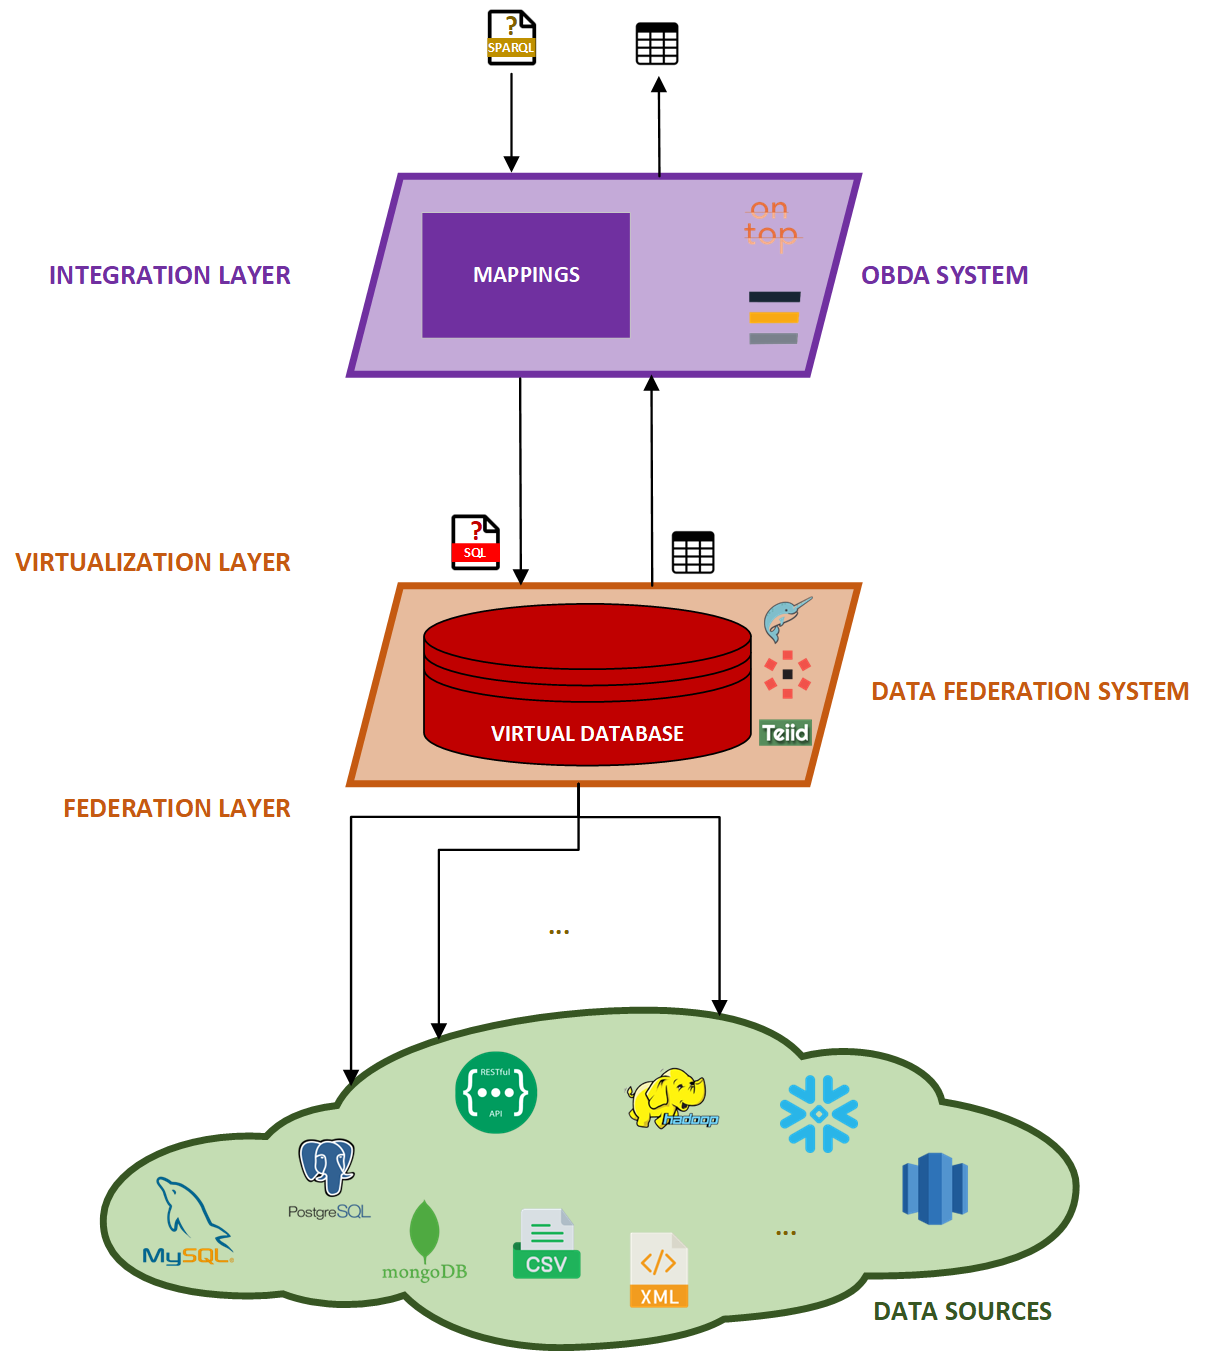
\includegraphics[width=10cm]{res/Drawing4.png}
    \caption{OBDF approach}
    \label{fig:obdf}
\end{figure}